\chapter{States of the World and Asset Pricing}

Assets give a \textit{payoff} $x_{t+1}$. In our focus on stocks, 
$x_{t+1} = p_{t+1} + d_{t+1}$, where $p_{t+1}$ is the 
price of the stock at time $t+1$ and $d_{t+1}$ 
is the dividend paid at time $t+1$.
$x_{t+1}$ is a random variable, like a coin-flip - we don't 
know at $t$ what it will be at $t+1$. But we can assign 
probabilities to the possible outcomes of $x_{t+1}$.
We can think of the \textit{randomness} of $x_{t+1}$ as being
due to the randomness of the \textit{state of the world} at $t+1$.
$x_{t+1}$ takes on different values in 
different \textit{states of the world}.
We have:

\begin{equation}
    E(x_{t+1}) = \sum_s \pi(s) x(s)
\end{equation}

where $E(x_{t+1})$ is the expected value of $x_{t+1}$,
$\pi(s)$ is the probability of state $s$, and $x(s)$ is the
value of $x_{t+1}$ in state $s$.

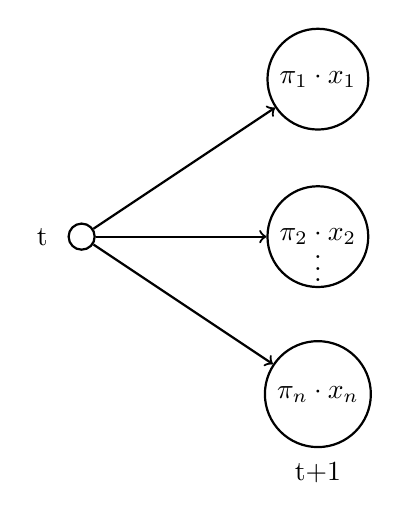
\begin{tikzpicture}[->, thick, auto, node distance=3cm]
    % Nodes at t
    \node[circle, draw] (t) at (0, 0) {};
    
    % Nodes at t+1
    \node[circle, draw] (t1s1) at (3, 2) {\(\pi_1 \cdot x_1\)};
    \node[circle, draw] (t1s2) at (3, 0) {\(\pi_2 \cdot x_2\)};
    \node[circle, draw] (t1sn) at (3, -2) {\(\pi_n \cdot x_n\)};

    % Edges
    \draw (t) -- (t1s1);
    \draw (t) -- (t1s2);
    \draw (t) -- (t1sn);
    
    % Labels for time
    \node at (-0.5, 0) {t};
    \node at (3, -3) {t+1};
    
    % Dots for multiple nodes
    \node at (3, -0.3) {\(\vdots\)};
\end{tikzpicture}